\documentclass[11pt]{book}
\usepackage{geometry}        
\geometry{letterpaper}    
\usepackage[parfill]{parskip}  
\usepackage{graphicx}
\usepackage{amssymb}
\usepackage{epstopdf}
\usepackage{listings}
\usepackage{adjustbox}
\usepackage{nameref}
\usepackage[toc, page]{appendix}

\DeclareGraphicsRule{.tif}{png}{.png}{`convert #1 `dirname #1`/`basename #1 .tif`.png}

\usepackage[colorlinks=true, pdfstartview=FitV, linkcolor=blue, 
            citecolor=blue, urlcolor=blue]{hyperref}
\usepackage{pgfplots}
\usepackage{float}
\restylefloat{table}


\newtheorem{theorem}{Theorem}
\newtheorem{corollary}[theorem]{Corollary}
\newtheorem{definition}{Definition}
\newtheorem{lemma}{Lemma}
\newtheorem{exercise}{Exercise}
\newtheorem{remark}{Remark}
\newtheorem{example}{Example}
\newtheorem{warning}{Warning}
\newcommand{\rhpc}{RHPC\_SMPLE }
\renewcommand{\lstlistingname}{Sample Code}

% Marin: This can be used to do the footnote = hyperlink in one step
\newcommand\footlink[1]{\footnote{\href{#1}{#1}}}

\def\grad{ \mbox{grad}}
\def\curl{ \mbox{curl}}
\def\div{ \mbox{div}}
\def\U{\ensuremath {\cal U}}
\def\S{\ensuremath {\cal S}}
\def\V{\ensuremath {\cal V}}
\def\R{\ensuremath {\cal R}}
\def\tr{\ensuremath {\mbox{tr}}}




% ------------------- Title and Author -----------------------------
\title{Repast HPC Social Media Platform Emulator \\(RHPC SMPLE)}
\author{User Guide}

\begin{document}


\frontmatter
\maketitle

\tableofcontents	

\mainmatter
%!TEX root =  RHPC_SMPLE_UsersManual.tex

\chapter[Introduction]{Introduction} \label{chap:Introduction}

Repast HPC Social Media Platform Emulator (RHPC SMPLE) is a toolkit for building agent-based models of behavior and information spread on social media platforms. The toolkit allows creation of a simulated social media platform with users who can engage with that platform, share content, and interact. The models created are agent-based models in the sense that the users who are interacting with the platform are agents and the platform itself is an agent. As agents, platforms can make decisions about what information they share among users; users as agents can make decisions about how they use the social media platform. The simulated platform can provide functionality representative of real-world social media platforms (e.g., posting, liking, rating, following, etc.). 

RHPC SMPLE is constructed from Repast HPC. Repast HPC is a toolkit for building large-scale agent-based models that can be parallelized for execution in high performance parallel computing environments. When an agent-based simulation is parallelized, the parallelism results in a challenge of keeping simulation states consistent across processes while allowing parallel execution of portions of the simulation on each process. Repast HPC handles the inter-process communication and synchronization issues in flexible and customizable ways while allowing the model developer to avoid writing low-level parallelization code. RHPC SMPLE is written in C++ to be usable on Top 500 HPC systems, potentially allowing social media simulations at real-world scales, i.e., millions or billions of agents.

\section{How to Use this Manual}

This manual provides a comprehensive guide to building social media emulators in \rhpc and to deploying and benchmarking these emulators. The guide consists of the following chapters:

% Marin- Pls make into itemized list, use chapter references and italics for all chapters as in the first one, and otherwise prettify as needed (make sure the titles are correct, etc.)
\begin{itemize}
\item Chapter \ref*{chap:Installation}, \hyperref[chap:Installation]{\textbf{Installation}}, provides technical details for installing RHPC\_SMPLE, including requirements and dependencies.
\item Chapter \ref*{chap:OverviewOfFunctionality}, \hyperref[chap:OverviewOfFunctionality]{\textbf{Overview of Functionality}}, provides a detailed description of the functionality of the \rhpc toolkit.
\item Chapter \ref*{chap:CodeStructure}, \hyperref[chap:CodeStructure]{\textbf{Code Structure}}, gives a tour of the source code for the toolkit and how it is organized.
%parallelization is an advanced topic and the simulation currently can't be parallelized easily, so this is a bit down the road...
%\item Chapter /href{Parallelization}, \textbf{Parallelization}, discusses the challenges of parallelizing an ABM and how these are addressed in the \rhpc toolkit.
\item Chapter \ref*{chap:CreateANewPlatform}, \hyperref[chap:CreateANewPlatform]{\textbf{Create a New Platform}}, gives step-by-step instructions for creating a new abstract social media platform in the \rhpc toolkit.
\item Chapter \ref*{chap:ExtendAPlatformToADemo}, \hyperref[chap:ExtendAPlatformToADemo]{\textbf{Extend a Platform to a Demo}}, gives instructions for creating a specific implementation of a social media platform in the \rhpc toolkit.
\item Chapter \ref*{chap:CreateUserAgents}, \hyperref[chap:CreateUserAgents]{\textbf{Create User Agents}}, describes how to create agents that use the implemented social media platform. 
\item Chapter \ref*{chap:CreateScenarios}, \hyperref[chap:CreateScenarios]{\textbf{Create Scenarios}}, gives instructions for how to create scenarios that encapsulate a specific use case for a model of one or more social media platforms, users, and exogenous events to which users and platforms respond. 
\item Chapter \ref*{chap:Output}, \hyperref[chap:Output]{\textbf{Output}}, discusses how to create structures that output to files.
\item Chapter \ref*{chap:LaunchingASimulation}, \hyperref[chap:LaunchingASimulation]{\textbf{Launching a Simulation}}, describes how to launch the simulation (including parallelized versions) and how to specify simulation options from the command line.
%\item Appendix \ref*{chap:Benchmarking}, \hyperref[chap:Benchmarking]{\textbf{Benchmarking}}, describes how to create performance tests at scale and in parallelized environments for strong and weak scaling tests.
\end{itemize}


\section{Acknowledgements}
%specific text that we have to use to acknowledge funders
%The funders (DARPA), the creators, the team, etc.
%!TEX root =  RHPC_SMPLE_UsersManual.tex

\chapter{Installation} \label{chap:Installation}

% Really this section needs to be resolved into separate sections:

%     Install MPI or confirm that it is already installed on your system
%     Install NetCDF or confirm that it is already installed on your system
%     Install the latest version of Boost (or confirm that it is already on your system)
%     Install Repast HPC on your system
%     Modify the rhpc_smple makefile.env file to point to the locations of these elements on your system
%     Invoke compilation using your MPI-provided compiler (or manually invoking MPI) 
%     If you are creating a new platform (not one of the pre-packaged ones) create a new implementation for your model; this is at the level of 'platform' in the demo directory.
%     Modify the equivalent of the social-sim.env file to point to the appropriate elements in your system
%     Compile and link to the appropriate libraries

Use of \rhpc requires the installation of the Repast HPC toolkit. Repast HPC carries three main requirements:

\begin{itemize} 
   \item \textbf{The Boost C++ Library}: the Boost\footlink{www.boost.org} library is a set of C++ extensions on which Repast HPC relies heavily; \rhpc is tested with versions up through 1.76.
   \item \textbf{NetCDF}: NetCDF\footlink{https://www.unidata.ucar.edu/software/netcdf/} is an extension to C++ that allows data read/write in a special dense format widely used in high-performance computing.
   \item \textbf{curl}: The curl library\footlink{https://curl.se/libcurl/} is a library that permits file transfers using multiple protocols.
\end{itemize}

Additionally, Repast HPC must be installed in a system that has an implementation of MPI (Message Passing Interface). MPI is a system that allows launching programs across multiple processes and manages the communication that occurs among these processes. Implementing MPI is a standard parallel processing operation, so any HPC system will likely have this installed; consult your system administrator. %to learn more? if not? if unsure? to download?
It may be possible to install MPI on a laptop, desktop, or AWS instance. Common implementations of MPI are OpenMPI\footlink{www.open-mpi.org} and MPICH\footlink{www.mpich.org}. 

Repast HPC can be installed by compiling against, and linking to, the Boost and NetCDF libraries and using your system's appropriate MPI compiler.

Once this is done, \rhpc can be installed by compiling against, and linking to, the Boost, NetCDF, and Repast libraries using the makefile included. To use this makefile, modify the file \textit{rhpc\_smple.env} and update the locations of Boost, NetCDF, and Repact HPC on your system. When this is built, it will create a new library, rhpc\_smple.lib. % CHECK THE NAME OF THE ENV FILE AND THE LIB

Once \rhpc is installed, you can compile using the header files in the \textit{include} directory, and build linking to the rhpc\_smple.lib library. % Check whether this a static or dynamic linking library?




%!TEX root =  RHPC_SMPLE_UsersManual.tex

\chapter{Overview of Functionality} \label{chap:OverviewOfFunctionality}

At a high level, the \rhpc toolkit allows creation of simulations of user behavior on social media platforms. Within this high level are a number of specific details that are summarized below.

\section{Overview}
The \rhpc toolkit is designed to create social media simulations that are conceptually structured as a set of concentric containers:

\begin{itemize}
\item At the outermost level is the \textbf{model}. A model is a runnable object that can be called by a c++ mainfunction. It executes the overall schedule of the simulation from start to completion.
\item Each model can contain a \textbf{scenario}. A scenario is a collection of social media platforms and any data that represent the real-world within which those platforms exist (e.g., world news events that will be discussed on the platforms). Scenarios can be nested so that a single scenario can contain multiple other scenarios.
\item A scenario contains one or more social media platforms.
\item Platforms contain nodes in a network. Generally, these nodes are of two types:
\begin{itemize}
   \item \textbf{Content nodes}, which represent posts to the social media platform, and
   \item \textbf{User nodes}, which represent user accounts on the social media platforms
\end{itemize}
\end{itemize}


\section{The Model}
The model is a container that wraps and guides the overall execution of the simulation. It handles the initialization of all the scenarios it contains (generally just one, but that one could potentially contain other nested scenarios; see below), the initialization of the simulation schedule, the overall management of time within the simulation, and any other required aspects of construction and tear-down.

Commonly, the model object is generic to a particular research project, and this can be written to contain multiple variant scenarios, all of which have time managed in the same way and all of which require similar schedules, initialization, and tear down, so that the scenario objects can be swapped in and out as needed.

\section{Scenarios}
Scenarios contain platform objects and representations of the real-world within which those platforms exist. The details of platform objects are discussed below. What is meant by the representation of the `real-world' can vary widely from project to project, but some examples could include:

\begin{itemize}
\item A time series of prices in some commodity, which agents on the platforms could then discuss
\item A set of news events that occur during the course of the simulation, which agents on the platform could respond to by increasing their activity levels
\item A time series of outages (accidental or intentional) that prevent some agents from participating in the discussion for periods during the simulation
\item A collection of specific pieces of information that would be available for discussion by the agents, and/or inserted into conversations on the platforms at specific times
\end{itemize}

In each of these cases, the scenario would be responsible for initializing the data structure that represents these items and for managing their statuses and changes during the operation of the simulation.

\subsection{Nested Scenarios}
A scenario can contain other scenarios. This employs several principles:

\begin{itemize}
\item The model object need only call methods like `initialize' on the outermost parent scenario; parent scenarios pass these downward to their child scenarios, so that all of them are initialized and operated in synchrony.
\item Information that is available to parent scenarios is also available to child scenarios.
\item Scenarios can be nested on-the-fly. At run time, a scenario can be designed and implemented such that it may or may not contain child scenarios so that tests can be run with and without the child scenarios. Scenarios can be designed once and re-used in different combinations.
\end{itemize}

The specific procedures to implement these are discussed in the technical documentation given below.

\section{Platforms}
The core of the \rhpc toolkit is the ability to construct a social media platforms. The Repast HPC paradigm for creating agent-based models relies on a core container object called a \textbf{context} which serves as the container for all kinds of agents\footnote{This conceptualization is derived from the Repast Java implementation but has a critical difference: in the Java version, contexts can be nested, so that one context can contain another; in Repast HPC this is not true, in part because contexts serve as the instrument for parallelization, a function that would be complicated by this nested structure.}. With a context exist one or more `projections', which contain the information about how agents are related to one another, either in a spatial relationship (e.g. a grid space) or connected in a network. In the \rhpc toolkit, a platform is a wrapper around a context and contains one core projection. The default implementation must only define the nodes that exist in this network, and the characteristics of the network's edges. Edges, for example, can contain `following' relationships among users, or `liking' relationships between users and content, or any other element that the platform needs to fulfill its set of functions.

These functions are constrained and specific, and they exist at two levels. At the generic level, platforms should be able to create new users\footnote{Platforms should also be able to create existing content nodes, especially if the operation is parallelized and the updates are to non-local nodes that are copied on the local process.}, and they should be able to respond to \textbf{queries}, which are requests for information about content or users on the platform. At the specific level, the platform should provide an \textbf{Application Programming Interface} (API) that user account agents can use to perform actions on the platform. These actions will include creating new content, forwarding or sharing existing content, etc., and should reflect the actions available in the real-world simulation being modeled\footnote{The degree to which an implementation of a specific platform's API reflects the real-world API of that platform is a design choice, and the implementation will not necessarily be fully equivalent to the real one.}.

The platform's agency---that is, its ability to be proactive and strategic in managing its relationships with its user accounts---comes from the fact that it is able to strategically respond to queries (by, for example, customizing the results it passes when a specific user account requests information) and that it can respond to requests to its API by making (or declining to make) changes to its network content. The latter can include tracking specific actions on specific content with information that can later be used to respond to queries in strategic ways. For example, if 100 accounts use the platform's API to indicate that they `like' a specific piece of content, then when a user account issues a query to see new content on the platform, the platform can select this popular piece of content over other new elements as a way to drive engagement. Later, it can respond by promoting other content produced by the same user account that originally produced the popular content.

% Internal team note (Don't put in text!): The fact that a platform = a context is one of the tricky parts about parallelizing a RHPC_SMPLE simulation, because RHPC wasn't really designed to have more than one context, so having more than one platform and parallelizing this can be, um, tricky...

\section{Social Media Network Nodes: Content and User Accounts}
Platforms are fundamentally wrappers for RHPC's network projections, and hence network nodes are central to its operation. The graph used is a directed graph. Nodes can be of two kinds: \textbf{content nodes} and \textbf{user accounts}. The network need not be strictly bipartite: links are possible between any two kinds of nodes; the most common may be links between users and content, but links from content to users, users to users, and content to content are all possible. The network can be used to track these relationships, for example:

\begin{itemize}
\item User A `liked' Content Z
\item User A `follows' User B
\item Content Z was created by User A
\item Content Z was a quote of Content Y
\end{itemize}

The development of network edges is a key aspect of creating a \rhpc simulation. The edge data structure should be able to capture these kinds of relationships\footnote{An advanced design can be employed that adds more than one network to a platform. This could be done for performance reasons, e.g. having a separate network that just stores content-to-content relationships may make searching for those relationships faster.} and make them available for use by the API and for responding to queries. 

\subsection{Social Media Content}
Content nodes represent pieces of content that users have posted on the social media platform. In the abstract, these are placeholders for any component that expresses a relationship among users; their main function is to link user accounts to other user accounts. Without any semantic association, this is the only things that a content node can do.

However, content nodes, in the abstract sense, can be endowed with a \textit{payload}, which represents real content: pieces of information that users can engage with or interact with, share and transmit, and respond to in specific ways. For example, a content node could be endowed with a true-or-false flag representing some issue that some agents are `for' while other agents are `against'. Content that is on one side of the issue may attract specific responses from some agents, and opposite responses from others; the platform can use this to strategically present agents with content of one kind or the other. Richer content (stance on multiple issues, combinations of specific pieces of information, or event full text) is possible; no real limitation is imposed by the \rhpc toolkit.

\subsection{Social Media User Accounts}
User accounts reflect entities on the social media platform that can respond to information and take action. Actions are undertaken via the API. User accounts are typically agents, with strategies, goals, memories, and other attributes that guide their interactions with the social media platforms and with the other accounts that they encounter through those media. The key element that the \rhpc toolkit is intended to simulate is how agents, pursuing these goals through their varying strategies, are able to use the social media platforms, and the resulting social structure and flow of information.

\subsubsection{People and Bots}
A specific technical issue in the above discussion is that user accounts on social media platforms are just that: accounts. 
Typically, these are considered to be `agents', and thus we conceive of them as individuals with memory, action, intent, strategy, or whatever other elements of the social simulation we want to use. However, an account is not a person. In some simulations, it may be preferable to create representations of real-world people; each person, then, can possess and act upon one or more social media accounts\footnote{It is also possible to have a single account that is shared among multiple people (such as different managers of a public-facing corporate account), but this is not discussed here.}. Strategies and other aspects of behavior, including offline interactions, could in this way be implemented across social media platforms, and user accounts would merely be tools that these person objects would use. This design choice may be specific to the project being undertaken. Because it is often difficult to fully link user accounts represented in social media data with real-world individuals who hold multiple accounts, the paradigm in which an account on a platform is the locus of agency (strategy, memory, etc.) is the more common case, but the use of person objects that possess multiple accounts is easily accommodated as well.

Bots, fortunately, are a simpler case, as there is essentially no distinction between a bot and a person, save that the capabilities and strategies of a bot may be very different. For example, a `person' might be implemented such that actions by that person are only undertaken during waking hours of the day, while a bot would have no similar restriction. Bots could in theory control multiple accounts, or they could be implemented as if they were equivalent to user accounts (with no separate `person' class possessing the account), as in the above discussion.

%!TEX root =  RHPC_SMPLE_UsersManual.tex

\chapter{Code Structure} \label{chap:CodeStructure}
The \rhpc toolkit distribution includes three major components, and this chapter provides a brief overview of the functionality of each:

\begin{itemize}
  \item \textbf{Social Network Tool Kit}: This is the core code that provides the fundamental functionality from which social media platform emulators can be built.
  \item \textbf{Platform Implementations}: This is a collection of platforms with proposed implementations built from the core code.
  \item \textbf{Demonstrations}: This is a collection of demonstrations constructed from the two components above.
\end{itemize} 

\section{Social Network Tool Kit}

\subsection{Utilities}
The \rhpc toolkit includes a small collection of utilities that permit common operations that are not specific to the simulation of online social media behavior but are also not provided in the standard Repast HPC code base. These include:


\begin{itemize}
% Marin: We may not leave this in the code- it's specific to SocialSim, but it's also in the DNA in the upper level code (unfortunately)
%  \item Standard definitions for file input formats (\textit{FixedOrderEventLog})
  \item Classes for performing weighted selection (\textit{SimpleWeightedSelector}, \textit{ParameterizedWeightedSelector})
  \item Standard definitions for return values for successful and unsuccessful completion and exit (\textit{ReturnValues})
  \item A class for writing output to files (\textit{FileWriter})
  \item Other utilities (\textit{Utilities})
\end{itemize}

\subsubsection{Weighted Selection}
Weighted selection is a common operation in simulations. 
For example, assume that there are ten agents that have an instance variable called `salary'. 
The goal is to simulate that agents with a higher salary may perform some action (e.g., buying a luxury item). 
The simulation to permitted to choose an agent randomly. 
If an even distribution is used for selection, every agent has an equal probability of being selected:

\begin{equation}
p_i = C
\end{equation}

where the probability of agent $i$ being selected is equal to $C$, a constant. However, suppose the selection is weighted based on salary, such that: 

\begin{equation}
p_i =  \frac{s_i}{\sum\limits_{a=1}^n s_a}
\end{equation}

That is, the probability of agent $i$ being selected is equal to that agent's salary divided by the sum of all agents' salaries. Assuming salaries of:

\begin{table}[H]
\begin{center}
\caption{Agents and Salaries}
\label{table:AgentsAndSalaries}
\begin{tabular}{l | r l}
\hline
 Agent & Salary \\
\hline
  Agent 1  & 20,000 \\
  Agent 2  & 10,000 \\
  Agent 3  &  5,000 \\
  Agent 4  &  5,000 \\
  Agent 5  &  5,000 \\
  Agent 6  &  5,000 \\
  Agent 7  &  5,000 \\
  Agent 8  &  5,000 \\
  Agent 9  &  5,000 \\
  Agent 10 & 5,000 \\
\end{tabular}
\end{center}
\end{table}

The relative probabilities of any agent being selected are easily calculated from the salary values: Agent 1 has twice the probability of being selected as Agent 2, and four times the probability of any of the other agents (3 through 10). In terms of absolute probability, Agent 1 has a probability of $\frac{2}{7}$; this is because the total salary is 70,000, and Agent 1 has 20,000 of this. The others' probabilities are $\frac{1}{7}$ for Agent 2, and half of this ($\frac{1}{14}$) for all other agents.

To achieve weighted selection in the \rhpc code, the SimpleWeightedSelector class can be used. The usage would be in three steps:

\begin{enumerate}
\item Create the instance.
\item Add elements to the instance in a specific sequence. The elements are the \textit{values} that should be used as weights. In the example above, this would be the salaries.
\item Request a selection; the value returned will be the \textit{position} (zero-indexed) in the list of values. 
\end{enumerate}

Importantly, the SimpleWeightedSelector takes only \textit{integers} as weights. 

The ParameterizedWeightedSelector operates exactly as a SimpleWeightedSelector after the values are added but allows parameters to be added that adjust the values as they are being input. This permits changes of several different kinds:

\begin{itemize}
\item An exponent can be added, such that the values that are put in are raised to a power. In the above example, this would cause Agents 1 and 2 to be even more heavily weighted. If the exponent was 2, then the weighting for Agent 1 would be 400,000,000; for Agent 2 it would be 100,000,000; and for all the others it would be 25,000,000. This means that the relative weight for Agent 1 would be increased from merely 4 times that of the lowest-salary agents to a factor of 16.
\item A scalar multiplier can be applied in the ParameterizedWeightedSelector. Doing so does \textit{not} change the relative weightings. Use this for cases where the original weightings are less than one; applying the multiplier transforms these weightings to integers (but truncates digits when doing so, which may make small distinctions between the weightings invisible).
\item The weighted selector allows the weightings to be adjusted after they have been initialized. One use of this is selection without replacement. If this is needed, then after the selection is made and the index of the selected element is returned, a call can be performed to \textit{clearat()}, which will re-set the weighting at that position to zero. Once the weight is zero, that element cannot be selected again.
\end{itemize}

\subsubsection{Return Values}
As a convenience, the toolkit provides a collection of constants that are used throughout the code as return values in the case of unsuccessful termination. Use the ReturnValues.h class as a reference to the meanings of these.

\subsubsection{FileWriter}
A generic class for writing output to files is provided here; see Chapter \ref{chap:Output} for more on writing to files.
\par \textbf{\textit{NOTE}}: This class is specific to the \rhpc toolkit. It is not a part of the social media structure, and utilities are not related specifically to the simulation of social media.

\subsubsection{Other Utilities}
One final class of utilities contains small set of functions that are used in the code. One is a helper function to extract a domain from a full web address. The others relate to setting properties with default values. See Chapter \ref{chap:CreateScenarios} to learn more about setting properties.

\subsection{Core Tools}

\par The core tools of the \rhpc toolkit are contained in the socialnetwork\_toolkit directories. There are 13 header files with four corresponding source files are present.   
They are shown in Table \ref{table:CoreToolkitFiles}:

\begin{table}[H]
\begin{center}
\caption{Core Toolkit Files}
\label{table:CoreToolkitFiles}
\begin{tabular}{l | l}
\hline
 Header & Source \\
\hline
 Action.h & \\
 BehaviorSelection.h & \\
 EdgeInformation.h & \\
 EventCounter.h & \\
 Explanation.h & \\
 Feed.h & \\
 InfoID.h & InfoID.cpp \\
 InfoIDSelection.h & \\
 InfoStore.h & InfoStore.cpp \\	
 Payload.h & Payload.cpp \\
 Scenario.h & Scenario.cpp \\
 SocialNetwork\_AbstractElement.h & \\
 SocialNetwork\_Platform.h & \\
\end{tabular}
\end{center}
\end{table}

The file listed in table \ref{table:CoreToolkitFiles}, and the classes they contain, fall into a few categories: 
\begin{itemize}  
\item There are the \textit{core elements} from which platforms and user agents are built:
   \begin{itemize}
	\item SocialNetwork\_AbstractElement 
	\item SocialNetwork\_Platform
	\item EdgeInformation 
	\item EventCounter
   \end{itemize}
\item There are the \textit{actions that these agents can take}, including content that these actions might convey:
    \begin{itemize}
	\item Action
	\item Payload 
   \end{itemize}
\item There are those that deal with units of information that agents may discuss (e.g., hashtags):
   \begin{itemize}
	\item InfoID
	\item InfoIDStore
	\item InfoIDSelection 
    \end{itemize}
\item  There are those that represent the collections of data shared from platforms to users (to which users respond), and any explanatory elements that get transmitted with these collections:
    \begin{itemize}
    	\item Feeds
	\item Explanations
   \end{itemize}
\item BehaviorSelection provides a generic structure by which user agents can choose behaviors
\item Scenarios are containers that include platforms and `real-world' elements and events to which agents and platforms may respond
\end{itemize}


\section{Platform Implementations}

\subsection{Twitter}
Twitter was founded in 2006 and is now one of the most widely used social media platforms in the world, with more than 192 million active users\footnote{\href{https://s22.q4cdn.com/826641620/files/doc_financials/2020/q4/FINAL-Q4'20-TWTR-Shareholder-Letter.pdf}{https://s22.q4cdn.com/826641620/files/doc\_financials/2020/q4/FINAL-Q4'20-TWTR-Shareholder-Letter.pdf} } and over 500 million messages posted every day\footnote{\href{https://www.dsayce.com/social-media/tweets-day/}{https://www.dsayce.com/social-media/tweets-day/} }.
\par Twitter is a microblogging platform that allows users to send and receive short posts. 
The length of these posts, which are called ``tweets", can be up to 140 characters long. In these tweets, users can include emojis, images, videos, and URLs. 
Original tweets can be ``retweeted", meaning information in a tweet from one user is shared by another user. 
Thus, retweeting is a quick and easy means of sharing information across wide audiences. 
A tweet has the capacity to reach a wide number of people. 
\par Another aspect of tweets are that they can be replied to and quoted. Replying and quoting aren ways of engaging with users by starting, or joining, conversations. 
Another means of engagement is the ``like" function. By liking, users can show acknowledgement, appreciation, or support for a tweet.
\par On the real Twitter platform, users can ``follow" other users. Following subscribes a user to another user's tweets. This means that a follower will be able to see tweets on their ``home timeline''. The home timeline shows all of the tweets from all followed users. From here, a user can like, reply, quote, or retweet. Another feature of the real Twitter platform is that it enables the followed and follower users to send direct messages to each other. 

\subsubsection {\rhpc Implementation}
\par In the \rhpc tool kit, users can undertake four actions: tweet, reply, quote, and retweet. There is no \textit{follow} functionality, nor is there anything akin to a \textit{like}.

\subsection{Telegram}
Founded in 2013, Telegram is a social media and instant messaging service meant for mass communication, but with a concern for privacy\footnote{\href{https://www.spglobal.com/marketintelligence/en/news-insights/latest-news-headlines/telegram-crosses-500-million-monthly-active-users-62094638}{https://www.spglobal.com/marketintelligence/en/news-insights/latest-news-headlines/telegram-crosses-500-million-monthly-active-users-62094638}}. 
As of January 2021, Telegram has over 500 million active users.
In 2021,Telegram was one of the most downloaded apps in Brazil, Malaysia, Russia, the Netherlands, India, Germany, the United Kingdom, Australia, and the United States\footnote{\href{https://backlinko.com/telegram-users}{https://backlinko.com/telegram-users}}.
In 2019, it was used for Hong Kong protests and by Islamic State extremists\footnote{\href{https://www.businessofapps.com/data/telegram-statistics/}{https://www.businessofapps.com/data/telegram-statistics/}}.
 \par One feature of Telegram is that it has secret chats. These are end-to-end encrypted conversations, meaning that the conversations are private and cannot be monitored. Telegram also allows file sharing that can be done through these secret, encrypted chats.
Another feature of Telegram is that it has private and public ``channels". These channels are groups where up to 200,000 users can communicate\footnote{\href{https://www.vox.com/recode/22238755/telegram-messaging-social-media-extremists}{https://www.businessofapps.com/data/telegram-statistics/}}. For private channels, users have to be invited and permitted to join.
 
The \rhpc implementation of Telegram is essentially identical to Twitter, save that the actions available are only 'post' and 'reply'.

\subsection{Reddit}
Founded in 2005, Reddit is a collection of forums for different topics. 
There are different communities for different topics, and each community is called a ``subreddit". 
It is the seventh most popular website in the United Sates{\footnote{\href{https://www.alexa.com/topsites/countries}{https://www.alexa.com/topsites/countries}} and the nineteenth most popular world-wide\footnote{\href{https://www.alexa.com/topsites}{https://www.alexa.com/topsites}}. 
Reddit is used for sharing content such as news, images videos, and text. 
These content types are posted to subreddits. 
There is a searchbar for searching key terms to find posts and subreddits to find content that relates to a given key term. It is also possible to search for users.
As of 2020, there were about 222 million active users{\footnote{\href{https://www.oberlo.com/blog/reddit-statistics}{https://www.oberlo.com/blog/reddit-statistics}}, and there are more than 46.7 million searchers a day \footnote{\href{https://foundationinc.co/lab/reddit-statistics/}{https://foundationinc.co/lab/reddit-statistics/}} due to the breadth of topics available on Reddit.
 \par ``Commenting" is a way of engaging with content and other users.
Comments can be responses to an original post or to other comments. When responding to a post or comment, it is possible for a user to ``quote" part of that comment for the purpose of specifying what is being responded to.
Also, similar to the ``like" function in Twitter, ``voting'' shows acknowledgement, appreciation, or support  via the ``upvote" function. 
This also increases visibility. 
However, there is also a ``downvote" function which is typically used  for when a post is not appropriate for a given subreddit, and this decreases visibility.
\par Subreddits tend to have their own rules for behavior that are enforced by moderators, or ``mods'', who volunteer to maintain the content and user behavior in the sub.
\par The homepage shows trending news posts from different subreddits, popular posts from different subreddits, and trending posts from the subreddits to which a user subscribes. A user can subscribe to other users too via the ``follow" function.
News can be sorted based on interests and date while popular posts from popular and user-selected subreddits can be sorted by upvote-to-downvote ratio, newness, and other features.
\par In the \rhpc tool kit's Reddit, users can post and comment. 
While the real Reddit has more user options, posting and commenting have been deemed the essential actions for understanding user behavior regarding spread of information. 

\subsection{Jamii Forums}
\par Founded in 2006, Jamii is a collection of forums for engaging in free discussions. 
Based in Tanzania, Jamii is known for its citizen journalism and for being an alternative news source. 
While there are a variety of forums for different topics, the popular forums discuss political, economic, and social issues as well as current events.
Jamii is the top most visited website for Swahili speakers around the world, and as such, it is most popular in East Africa\footnote{\href{https://www.zoomtanzania.com/company/jamii-forums}{https://www.zoomtanzania.com/company/jamii-forums}}. 
As of August 2017, there were ``more than 2.4 Million users, 28 Million mobile subscribers and up to 600,000 people using its online forum daily"\footnote{\href{https://tanzania.mom-rsf.org/en/owners/companies/detail/company//jamii-media-co-limited-1/}{https://tanzania.mom-rsf.org/en/owners/companies/detail/company//jamii-media-co-limited-1/}}.
 More recently, on June 25, 2020 at 11:42 AM CT, there were 1,554,248 threads, 38,986,717 messages, and 575,354 users\footnote{\href{https://www.jamiiforums.com}{https://www.jamiiforums.com}}.
\par The homepage consists of lists of forums. 
From here, it is possible to create new posts, search forums for key terms or users, see new posts and recent activity of other users, and see lists of online users. 
\par Like Reddit, ``commenting" is a way of engaging with content and other users.
Comments can be responses to an original post or to other comments. 
When responding to a post or comment, it is possible for a user to ``quote" part of that comment for the purpose of specifying what is being responded to.
Also, just as with the ``like" function in Twitter, users can engage with other users and their content via the ``like" function.
By liking, users can show acknowledgement, appreciation, or support for a post or comment.

The \rhpc implementation of Jamii currently allows only posts, which initiate a thread within a forum, and comments, which belong to that thread. Quoting, which would have the effect of enabling one post to reply directly to another, is not implemented. 

\textbf{\textit{NOTE}}: As a technical detail, the \rhpc Jamii implementation differs from the Reddit implementation in one important way: As a way to ensure performance at very large scales, the Reddit implementation does not treat all content as `first class' content nodes. Instead, all `posts' are full nodes, but `comments' are recorded only as partial records- essentially a notation that something happened, but not a full record of the event. These notes descend from posts in a tree structure (comments of comments), but comments cannot be directly selected as targets of actions. The performance enhancement that this offers is mainly speed in selecting targets, as well as some reduction in the memory footprint of the simulation.

\subsection{YouTube}
Founded in 2005, YouTube is a site for sharing videos comprised of original content. The most popular types of videos are tutorials, comedy, and music\footnote{\href{https://www.thinkwithgoogle.com/consumer-insights/consumer-trends/top-content-categories-youtube/}{https://www.thinkwithgoogle.com/consumer-insights/consumer-trends/top-content-categories-youtube/}}, but there are other popular genres too. Users can also livestream to other users in real time.
YouTube is popular worldwide and has local versions for over 100 countries and has over 2 billion regular users. Everyday, users watch ``over a billion hours of video and generate billions of views" \footnote{\href{https://www.youtube.com/intl/en-GB/about/press/}{https://www.youtube.com/intl/en-GB/about/press/}}.
Additionally, YouTube averages 100 hours of uploaded video per minute{\footnote{\href{https://edu.gcfglobal.org/en/youtube/what-is-youtube/1/}{https://edu.gcfglobal.org/en/youtube/what-is-youtube/1/}}. Videos often have closed-captions that can even be available in multiple languages.
Aside from hosting videos, YouTube has features that render it a social media platform. Each ``channel" on YouTube is a user's account. Users can subscribe to other users' channels to stay up to date on other users' content. There is also a ``comment" function so that users can comment on videos and reply to other comments. \footnote{However, there is a difficulty in the user interface where people reply as if they are replying to the comment above theirs, but this is actually not the case. This means that there is a reply structure between posts that, in terms of content, should be at the same structural level}.
Additionally, users can ``like" videos and comments to show acknowledgement, appreciation, or support. Liking boosts the popularity, and therefore visibility, of comments and videos. 
\par On the homepage are recommended videos based on subscriptions as well as those that the platform thinks the user would like. There is also a section for news videos. 

\subsection{GitHub}
Founded in 2007, GitHub is a leading code-sharing site. While not a traditional social media site, it is nevertheless a place where people interact online: "Millions of developers and companies build, ship, and maintain their software on GitHub" with over sixty-five million developers and over three million organizations involved \footnote{https://github.com/about}. 
\par The major features of GitHub are that it enables collaboration and maintaining version control for coding projects. Collaboration involves  four main processes:
\begin{itemize}
\item Creation and usage of a `repository' of any and all project parts. This can include data sets, folders, files, images, videos, etc. 
\item Creation and management of a `branch'. There is always a `main' branch. Branches are used to experiment with changes before `committing' them to the main branch. 
\item Commits are the way to make changes to a file that are shared across people in a project. Commits are `pushed' to finalize the changes made within a branch.
\item Pull requests can be opened for merging branches. Making a `pull request' means proposing the contributions a user has made for review so that the changes can be merged into a branch. The @mention system can be used in a pull request message for feedback requests.
\end{itemize}

% Other actions people can take on GH?
%What does our tool kit do?




\section{Demonstrations}

\subsection{Demonstration Platform Implementations}

\subsubsection{Foobook}

\subsubsection{Pingstagram}

\subsection{Demonstration Scenarios}

\subsubsection{Scenario 1: Basic Foobook}
This is the test used for \nameref{chap:Benchmarking}.

\subsubsection{Scenario 2: Foobook with Malicious Users}

\subsubsection{Scenario 3: Foobook and Pingstagram}

\subsubsection{Scenario 4: Foobook and Pingstagram with Coordinated Users}


%%!TEX root =  RHPC_SMPLE_UsersManual.tex

\chapter{Parallelization} \label{chap:Parallelization}
\textbf{Parallelization} is the division of a single computational problem across multiple processors. The operation can be anything from a simple but very large mathematical operation to a complex simulation. The goal of parallelization is to reduce the real-world time of solving the problem the simulation is meant to address. In the ideal case, the time to solve the problem is changed from $T$ to $\frac{T}{N}$, where $N$ is the number of processors across which the problem is divided. For example, if it takes 10 minutes to add a billion numbers together on one processor, then if the problem is divided across 10 processors, it could theoretically be solved in one minute.

In practice, the performance gain is never this perfect: although the computational time might be reduced linearly based on the number of processors, the act of parallelization imposes some additional costs. In the case of the simple addition problem above, we can assume that the billion numbers are stored on one of the processors at the start, and that this same processor is the one that needs the sum at the end. In this case, the overhead comes because the process needs to divide up and distribute the data across the ten processes (presumably itself and the other nine processes), and then receive the sums back from the other nine processes, and finally perform the last addition in which those sums are added together to get the final result.

However, this idealized case is very far from the situation that occurs when parallelizing an agent-based model. In the case of the simple addition problem, each of the processes can act independently because the result that would be obtained on one process does not depend on the results from any other process. Consequently, each process can perform the operation without any interaction with the other processes. However, in an agent-based model, where the critical aspect of the simulation being tested is the way that the agents interact, the potential for cross-process dependencies is very high.

A common example is agents positioned on a grid and moving such that each agent takes a turn in which it chooses a direction and moves some number of grid squares. A very common corollary in this kind of simulation is that a grid square can be occupied only by one agent at a time. Consequently, the requirement that the agents take turns is crucial: if only one agent is acting at a time, then it can assess which squares around it are empty and move into any empty square without violating the rule.

This simple state of affairs becomes significantly more complicated when the simulation is parallelized and agents are acting on more than one process simultaneously. If this is the case, it is possible for an agent to be unsure if a particular grid square is empty or not: it might be possible for an agent on another process to also be considering that square as a destination, or even to have moved there already. If the information that the square is occupied has not traveled from one process to another, the agent on the second process may not know that the agent from the first process has moved and the square is now taken.

In the worst-case scenario, this would create a chain of cascading dependencies: an agent would poll another process and/or negotiate with another process to determine which agent would act first, but all other agents with actions that might be impacted by this negotiation might also have to wait for it to be resolved. This could involve immediately neighboring agents waiting for their opportunities to move, which would cause their neighbors a few steps away to also have to wait, etc. It is even possible that the only resolution to this would be to impose a global control mechanism that would designate one agent across processes and allow that agent to act, effectively eliminating parallelization and its advantages. \footnote{In other contexts, solutions to this problem can reach extraordinary lengths: For example, `optimistic' approaches would have the agent move into the square and would merely make a note that it could be occupied. They would then continue allowing all other agents on that process to move. If information was later received that the square was occupied and the move into it was invalid, the entire simulation is then `rolled back' to the point where the collision occurred. The cost of the rollback can be high, but if it is rare and the benefit of moving ahead is great, then this strategy might be efficient.}

Because there is a need to establish some reconciliation process for cases like this, parallelizing ABMs is non-trivial. The main question to be faced is whether the reconciliation process imposed as a necessity to perform parallel operations is one that keeps the outcome of the simulation valid---that is, that parallelization does not make the simulation produce results that are not usable. In fact, of course, the strategy for implementing agent behaviors on a single process must also address this question, because the real world is parallel but the simulation is not; parallelization does not change this, but it does throw the question into the spotlight, because many tried-and-true strategies in serial environments (e.g., agents taking turns) do not work in parallel ones.

\subsection{When not to parallelize}

Parallelization of agent-based models faces an additional practical challenge. It is very good to take the simulation run time and reduce it by some factor, and if that factor approaches $\frac{1}{N}$ for $N$ processes, this can be an important gain. However, agent-based models typically rely on stochastic repetitions of runs so that the simulation is not run once, but multiple times, creating a range of results and a measurable distribution. Moreover, these are often conducted hand-in-hand with tests that involve multiple varying parameters. Consequently, the simulation must be run some number of times. The issue can be seen when assuming that this number is also $N$: if there are $N$ processors, the simulation can be made to run in $\frac{1}{N}$ time by using all of the processors. 
However, if needing to then run $N$ repetitions, it will take just as long to complete all of these as it would if all these runs were started as independent processes run simultaneously on all available processors. In general, the number of runs needed is much larger than the number of processors available, and so the overhead of running the simulation in parallel---as well as the extra development time to parallelize it---is better off avoided, and the runs should simply be done as independent, single-process runs.

There is, however, one exception to this: parallelizing a simulation also allows it to be divided up in \textit{size} as well as time. If a simulation is too large to be run on the memory available to a single process, then parallelizing it may be a solution. In the not-too-distant past, processes with 16GB, or even 8GB were the norm on even very large `supercomputers', and consequently a simulation that exceeded this, which was not uncommon, would need to be run on more than one process. Today, however, processes are available that have hundreds of GB of memory, enough to accommodate very large ABMs.

\section{Synchronization}
As discussed in the previous section, parallelization involves processes acting independently. As one process modifies the state of the simulation (e.g., by allowing an agent to move), other processes are temporarily unaware of this modification. This is what causes the difficulty with dependencies discussed above. The delay in updating the information from one process to another is termed being out of synchronization. It is intentional---it is what allows the processes to work independently\footnote{The general paradigm here is processes that do not share memory---in some systems, separate processes can share memory and this would seem to allow all processes to have access to the up-to-date simulation information. However, there could still be collisions and problems. For example, one process reads that the grid square is `empty' and then begins to perform the operation of letting another agent decide whether to occupy it, and while this is underway, another process moves an agent into that square. Direct access to memory does not resolve the basic issue, which derives from the parallelization.}. However, it raises an important design consideration: when does the simulation need to share information back across the processes?

This could be done on an ad hoc basis in some cases, but generally the assumption is that the processes will be allowed to run independently and then a global synchronization operation will be performed. This is the paradigm supported in the Repast HPC toolkit.

However, there are three \textit{different} kinds of synchronization that can be performed. They derive from the underlying paradigm that Repast HPC uses for parallelism. There are two crucial components to this paradigm:

First, the simulation tracks two different kinds of information about the agents: agent \textit{state} refers to the internal variables that an agent has (like salary, fuel, emotional level, etc.), and is internal to each agent; agent \textit{relationships} are tracked separately. Relationships can be of two kinds: networks, in which any agent can have a relationship with any other agents, and locations in a cartesian space. Location in space might initially seem to be an attribute of the agent, but in fact the location of an agent in absolute terms (e.g., at grid point $x=390, y=257$) only has meaning with respect to other things in the simulation\footnote{This is akin to the ability to choose different frames of reference; one can choose any point in the space and call it x=0, y=0, and this should not change the outcome of the simulation.}.

Second, the simulation is aware that agents exist on specific processes; agent 1 may have its `home' on Process 0. However, if agent 1 has a relationship with an agent on another process- for example, being close to it in space or being linked to it in a network- then Repast HPC will provide that process a copy of agent 1. This will allow the other agent to interact with agent 1. This copy is referred to as a \textit{non-local} agent, or sometimes (informally) a \textit{ghost agent}. The fact that an agent is local to a specific process is called that agent's \textit{status}. All relationships are kept in structures that are termed \textit{projections}.

This leads to the three kinds of synchronization:

\begin{itemize}
\item \textbf{Synchronization of Agent State} means updating the internal states of all non-local agents
\item \textbf{Synchronization of Projections} means updating the relationships an agent is involved in, including movement in space.
\item \textbf{Synchronization of Agent Status} means updating the status of an agent.
\end{itemize}

The first of these is the simplest: synchronizing agent states means copying the up-to-date information from the agents' home processes into the copies on other processes. Suppose Agent 1 is local to Process 0, and initially has an account balance of \$100. A copy is needed on Process 1, and this copy also initially has an account balance of \$100. But, during a time tick, the agent wins the lottery, and its account balance goes to \$30,000. For a period of time, the agent locally has the higher balance, but the non-local copy does not. Synchronizing the agent state copies the new balance into the copy of the agent on Process 1.

While this is the simplest kind of synchronization, it also imposes the hardest constraint: \textit{Information flows from home processes to non-local processes, but \textbf{never the other direction}}. Because of this, no change to the account balance of the `ghost' copy of Agent 0 on Process 1 should ever be made. The rationale for this is simple: the same agent may be copied as a `ghost' to multiple other processes, and updates made to all of these can't be reconciled. If something were happening on Process 1 that would affect the account balance, the correct way to do this would be to bring the information from Process 1 (including any other agents) back to Process 0, and have the interaction that makes the change take place there.

The synchronization of projections is more complicated, but a simple example can convey the basics. Supposed an agent is in a simulation with a grid space, and is near the edge of the space that the local process controls (say, the agent is at x = 99, with the boundary at x = 100). The adjacent process has the ability to perceive 3 grid spaces into this one; hence this agent is visible to the other process, where it appears as a non-local agent at x = 99. During the tick, this agent moves back a step, to x = 98. The copy on the other process remains at x = 99 until projection information is synchronized. When projection information is synchronized, the agent's new position at x = 98 is available to the other process via the non-local copy.

Note that these two operations can be done independently: the position can be changed without updating the account balance (internal state). Repast HPC does not require that they both be performed. Because these are computationally intensive operations, you can choose to do one without doing the other. If, for example, you know that account balances have been updated but no positions have been changed, then there is no need to update both elements.

Synchronization of agent status is more challenging because it has more possible variations. Two common ones are:

\begin{itemize}
\item A case in which an agent was local to Process 0 and had a non-local copy on Process 1, but which for some reason (for example, moving from x = 99 to x = 101, thus crossing the boundary into the space controlled by the adjacent process) must be moved so that it becomes local on Process 1. In this case, the original on Process 0 might become a `ghost' copy, while the copy on Process 1 becomes a full agent.
\item A case in which an agent local to Process 0, with non-local copies on other processes, is removed entirely from the simulation (e.g., `dies'). While the simulation is out of synchronization, the non-local copies persist; once agent status is synchronized, the non-local copies are all removed.
\end{itemize}

\section {Building and Running Parallel Simulations in RHPC SMPL}
%!TEX root =  RHPC_SMPLE_UsersManual.tex

\chapter{Create a New Platform} \label{chap:CreateANewPlatform}

\par The main purpose of the \rhpc toolkit is to allow the creation of a functionally faithful representation of a social media platform. The first step in this is the creation of a new platform object. In general, the practice is to create the platform abstractly at an upper level of implementation, and to do so in a way that allows a second customizable level. The upper level captures the known functionality of the platform, while the lower level permits the implementation of the user and platform behavior that is the object of some specific line of research. For example, the upper level may permit a piece of content to be `liked,' while the lower level provides implementations that allow user agents to decide which content elements they will perform this action on.

This chapter gives instructions on how to do create the abstract objects at the upper level of the implementation. The overall sequence is:

\begin{enumerate}
	\item Create all Header and Source Files
	\item Create Definitions for Required Elements
	\item Create Feed 
	\item Create Abstract Versions of Agent, User Agent and Content Agent
		\begin{itemize} \item Agent Type \item Action Type \item Relationship Type \end{itemize}
	\item Create a Payload Object
	\item Create an Action Object
	\item Create Required Network Elements
	\begin{itemize} \item Edge Information Objects \item Edges \end{itemize}
	\item Feed Query
	\item Create a Platform Using the Above Objects
\end{enumerate}

\section{Step 1: Create All Header and Source Files}
The platform code will require a version of all of the files shown in Table \ref{table:PlatformRequiredFiles}. Note that while some occur in pairs of header and source files, others need only header files.

\begin{table}[H]
\begin{center}
\caption{Files required to implement a new platform}
\label{table:PlatformRequiredFiles}
\begin{tabular}{l | l}
\hline
 Header Files & Source Files \\
\hline
 Definitions.h & \\
 Feed.h & Feed.cpp \\
 Agent.h & \\
 UserAgent.h & UserAgent.cpp \\
 ContentAgent.h &  \\
 Payload.h & Payload.cpp \\
 Action.h & Action.cpp \\
 Network.h & \\	
 FeedQuery.h & FeedQuery.cpp \\
 Platform.h & \\
\end{tabular}
\end{center}
\end{table}

Files can have different names than those shown here, e.g. customized for a particular platform. For example, ``UserAgent.cpp" could be named ``FoobookUserAccount.cpp". 

\subsection{Step 2: Create Definitions for Required Elements}
Creating \textbf{definitions} is done by modifying \emph{Definitions.h}. At this level, three elements must be defined:

\begin{enumerate}
\item Agent types
\item Action types
\item Relationship types (if applicable)
\end{enumerate}

Additionally, this file must provide a forward declaration for the class that will be the platform, such as in the example below.
% TODO: which file? is this actually shown in the upcoming example, or am I assuming?
% This may be revised- we would like to remove these forward declarations

The example below defines two types of \textbf{agents}, \textit{users} and \textit{content }(termed `posts'). It also defines two types of \textbf{actions}: one begins a new thread and the other posts to a given thread. No relationships are defined in this example. 

\input{CreateANewPlatform/code_examples/Code_Example_1_1.txt}
	
\subsection{Step 3: Create the Feed Architecture}
A \textbf{feed} is, fundamentally, a list of elements. It is similar to the `feed' that a user of a social media platform provides via the user interface (for example, friends' recent posts on Facebook). 

In \rhpc, a feed can also contain an \textit{explanation} of why each element was placed into it.  A typical definition of the feed begins by declaring the class that contains this explanation (if needed). 

Example:
\input{CreateANewPlatform/code_examples/Code_Example_1_2.txt}

In the above example, the \textit{explanation} is simple: a flag indicates whether or not the element was randomly selected.

Note that the second constructor is \textbf{required}. A copy instructor is needed because explanations are transferred among feeds and copied.

After the explanation, the \textbf{element} in the feed must be defined:

\input{CreateANewPlatform/code_examples/Code_Example_1_3.txt}

Finally, the \textbf{feed} itself must be defined:

\input{CreateANewPlatform/code_examples/Code_Example_1_4.txt}

Note that this implementation provides some methods that are used to select elements from the feed.
% Internal note: We are likely to remove this when we move to the Feed Explanation being optional;
% the change will allow the Feed to become a typedef, possibly eliminating the class altogther

\subsection{Step 4: Create Abstract Versions of Agent, User Agent and Content Agent}
As an agent-based model (ABM), agents are fundamental. In \rhpc, there are two kinds of agents: there are agents that represent \emph{users} (\textbf{user agents}) and agents that represent \emph{content} (\textbf{content agents}).

Both of these derive from a single abstract class that is the basic \textbf{agent class} in the RHPC content and the fundamental `node' element in the RHPC network.

\subsubsection{Step 4.1: Create the Abstract Version of the Agent}
At this level, the \textbf{agent class} needs only to be defined abstractly. Templatize the agent class to accommodate an action type that will not be specified until lower in the class hierarchy.

Example:
\input{CreateANewPlatform/code_examples/Code_Example_1_5.txt}
The individual procedures that the agent implements are:

\begin{itemize}
\item setCurrentRank(int):
\item showName():
\item writeName():
\item placeInFeed(actor*, target*, subtarget*, action, explanation):
\item setPlatform(platform*):
\item getCountOfFeedElements():
\item selectTarget(action\&):
\end{itemize}

\subsubsection{Step 4.2: Create the Abstract Version of the User Agent}
An important aspect of \textbf{user agents} is that they represent \textit{user accounts}. This is not the same as representing \textit{users}. Users are people, and people can use multiple social media platforms (sometimes simultaneously!). User accounts, conversely, are platform-specific. They can perceive only things on that platform and can only take actions that the platform defines.


Most user functionality is defined at the implementation level. Below this level in the class hierarchy, so the class need not hold much functionality. In fact, class is used below only as a demonstration.
%Note: We may change this: Jamii accounts have reputation scores, and while we don't fully understand these yet, it's appropriate to add them here.

Example:
\input{CreateANewPlatform/code_examples/Code_Example_1_6.txt}

\subsubsection{Step 4.3: Create the Abstract Version of the Content Agent}
\textbf{Content agents} can be more robustly defined at this level than user agents can be.

In the example below, the content agent has been endowed with a way to collect \textit{Information ID}values in the \textit{informationIDs} set.

Example:
\input{CreateANewPlatform/code_examples/Code_Example_1_7.txt}

The content agent is further specified by the \textit{receiveAction} method. This method is \textbf{required} because it allows content agents to be acted upon by users. 

The example below defines one critical piece of functionality, which is receiving the Information ID values and storing them in the set:

\input{CreateANewPlatform/code_examples/Code_Example_1_8.txt}

\subsection{Step 5: Create the Base Class for the Payload}
A \textbf{payload} is a package of data that is shipped with an action; an action will contain a payload, and the payload will be the `stuff' that an action includes.%revisit

Generally, the payload object represents the genuine \textit{content} portion of the content object. If a content agent contains elements like an ID, references to the user agent that created it, etc., it will also contain some content. This will be domain-specific but could include anything that is relevant in a given simulation: text, hashtags, abstract pieces of information, etc.

% Note: The Jamii implementation is currently another empty filler class, but we may extend this with a 'reaction'...

\subsection{Step 6: Create the Action}
As with a feed, an \textbf{action} can carry information that explains why the action was taken. Therefore the first component of an action is an \textit{ActionExplanation}.

Example:
\input{CreateANewPlatform/code_examples/Code_Example_1_9.txt}
%Note: 'headings' is going to be eliminated, as will 'getRow()', this note also in 'Code_Example_1_9.txt'

In the above example, the only portion of the explanation is \textit{becauseOtherUsersLiked}, which is a placeholder for more informative flags. Note that the \emph{Action Explanation} extends, and therefore contains, the \textit{FeedExplanation} defined above. Both of these are therefore extensions of \textbf{explanation}, which carries with it some inherent functionality (especially the ability to take one explanation and `add' it to another by performing a logical `or' on all boolean flags, etc.


Example:
\input{CreateANewPlatform/code_examples/Code_Example_1_10.txt}

%The significant procedure is getOutputRepresentation. The documentation should indicate that this is required, but that the actual output will be determined by the file output type, and this not defined at this level, but will be implemented at the lower/ "implementation" level.

\input{CreateANewPlatform/code_examples/Code_Example_1_11.txt}

\subsection{Step 7: Create Required Network Elements}
Defining a network involves defining \emph{flags}, \emph{counters}, and \emph{relationships}. The example below shows only counters. \textbf{Flags} are y/n and are used for things like ``X created Y" (true/false). \textbf{Counters} are used to count events (e.g., "1,234 likes").

Below is an example of a basic counter that can count the number of Jamii events that occur between two agents.

\input{CreateANewPlatform/code_examples/Code_Example_1_12.txt}

\subsubsection{Step 7.1: Edge Information Objects}
Counters can use these to make \textbf{edge information} objects. An edge information object stores a directed edge from two agents (e.g., from A to B). This is used in conjunction with flags/counters/relationships to indicate how A is related to B (e.g., ``A has 'liked' B 6 times).

To implement this, extend the appropriate class:

\input{CreateANewPlatform/code_examples/Code_Example_1_13.txt}

\subsubsection{Step 7.2: Edges}

After implementation, you can create an \textbf{edge} that contains the \textit{edge Information} object. This allows declaring a formal interface that can capture the appropriate semantics for the platform you are creating.
\par Note that /emph{getNumPosts} is not intrinsic to \rhpc, but rather is defined by the fact that in Jamii there are 'Posts'. 

\input{CreateANewPlatform/code_examples/Code_Example_1_14.txt}

\subsection{Step 8: Create a structure for a Feed Query}
A \textbf{feed query} is a class that contains the information needed for the platform to execute a query. In other words, it is a a set of criteria used to return a collection of content objects.

The feed query can be a simple structure.
\par Example:
\input{CreateANewPlatform/code_examples/Code_Example_1_15.txt}

\subsection{Step 9: Create a Platform Using the Above Objects}

A platform must:
\begin{enumerate} 
	\item Allow creating and updating \textbf{user agents} and \textbf{content agents}
	\begin{itemize} \item This includes setting local pointers \end{itemize}
	\item Allow responding to \textbf{feed queries} by providing feeds that include relevant items
	\item Allow performing \textbf{actions} from user accounts onto user or content nodes
\end{enumerate}

At this level, \textit{creating and updating} are not yet implemented. Implementation will happen at the lower level. Additionally, the responses to queries are not defined at this level; this is instead application-specific.

Instead, the actions to be performed for the \textbf{API} (Application Programming Interface) are defined at this level. The API is a list of functions that a piece of software (or a social media platform) can perform.

For Jamii,  the only actions are `post' and `comment' (see the definitions above). The relevant sections in the platform interface are:

\begin{lstlisting}
// API Functions
void doAction(ACTIONTYPE action);
void api_startThread(ACTIONTYPE action);
void api_comment(ACTIONTYPE action);
\end{lstlisting} 

In this case, the first is generic and should pass to the appropriate semantic operation based on the action passed. The `startThread' and `comment' actions represent `posting' and `commenting.'

Several other components of the platform may be defined at this level; look at the examples provided for details.


%!TEX root =  RHPC_SMPLE_UsersManual.tex

\chapter{Extend a Platform to a Demo}\label{chap:ExtendAPlatformToADemo}
The previous chapter outlined the steps required to use the \rhpc  toolkit to create a social media platform at an abstract level, capturing the basic functionality of the platform at the upper level while leaving the specifics for implementation at a lower level. These specifics could include, for example, agent behavior representing user accounts that interact with the platform's functionality in ways that are customized to the research question being explored.

This implies a second step: %to what exactly, the example from the previous paragraph?
the implementation of this lower level, so that the toolkit can be used to run simulations of online behavior. This chapter presents the steps necessary for running simulations.

\section{Hierarchy of Functionality}
Before discussing the step-by-step functions, a conceptual diagram of a relationship is presented to show the relationships among the classes declared in the previous chapter and the classes that will be discussed and implemented here. 
Figure \ref{TBD} shows these relationships.%

\section{Step-by-Step Instructions}
Below is a list of instructions. Each step is explained in the next section.
\begin{enumerate}
	\item Create all the Header and Source Files (empty)
	\item Create a makefile that compiles all source files
	\item Populate the Header Files
	\begin{itemize}
  	  \item Definitions
	  \item Agent Package
	  \item Custom Action
	  \item Agent
	  \item Content Agent
	  \item Behavior Selection
	  \item InfoIDSelector
	  \item User Agent
	  \item FileWriter
	  \item Feed Query
	  \item Platform
	\end{itemize}
	\item Populate the Source Files 
	\begin{itemize}
	  \item Package
	  \item Action
	  \item Agent
	  \item Content
	  \item Behavior
	  \item User
	  \item Feed Query
	  \item Platform
      \end{itemize}
\end{enumerate}

\subsection{Create all the Source and Header Files}
A good first step is to simply create the (empty) files as listed in the table.

\begin{table}
\label{table:ImplementationRequiredFiles}
\begin{center}
\caption{Files requred to implement a platform }
\begin{tabular}{l | l}
\hline
 Header Files & Source Files \\
\hline
 Definitions.h & \\
 Action.h & Action.cpp \\
 Agent\_Package.h & Agent\_Package.cpp \\
 Agent.h & Agent.cpp \\
 ContentAgent.h & ContentAgent.cpp\\
 UserAgent.h & UserAgent.cpp\\
 BehaviorSelection.h & BehaviorSelection.cpp\\
 FeedQuery.h & FeedQuery.cpp \\
 FileWriter.h & \\
 InfoIDSelection.h & \\
 Platform.h & \\
\end{tabular}
\end{center}
\end{table}



\subsection{Create the Definitions for File Output Type}
Here you should define a set of types that will be used to score agents when their order of retrieval is being determined.

If any file output is needed, then a definition of output type is required. See Chapter \ref{chap:Output} for more information. 

\textit{See Twitter\_Definitions\_xamples.h for an example of both of these.}

\subsection{Create the Agent Package}
The agent package should include all information needed to construct an identical copy of an agent.

\textit{See Twitter\_Agent\_Package\_xamples.h for an example of both of these.}

\subsection{Create the Abstract Agent, the User Agent, and the Content Agent}
The agent will inherit from the abstract agent, and will include any functionality that a general agent on this platform (whether user or content) should have. It will be templated by Action (from the platform level) and Score Type from the definitions at this level. \textit{See Twitter\_Agent\_xamples.h for an example.}

\subsubsection {User Agent}
\par The user agent will descend from the abstract user agent at the platform level and the agent at the demo level, and must implement selectBehavior, selectTarget, and selectInfoIDs methods. \textit{See Twitter\_Agent\_User\_xamples.h for an example; this example omits the inheritance of the demo level agent, but it is not needed for the demo.}

\subsubsection {Content Agent}
\par The content agent will descend from the abstract agent at the platform level and from the agent at the demo level. 

The content agent must implement two significant methods:

\begin{itemize}
\item \textit{receiveAction} This must process an action when this content target is acted upon. This includes any modification to the state of the target and any changes to the action.
\item \textit{getSelfPointer} This must return a pointer to self; it is used in specific situations where the pointer must be to the lowest child class but is generated by the parent. 
\end{itemize}

\par This structure allows the user agents and content agents to inherit demo specific behavior but avoids a diamond inheritance pattern with the objects at the platform level.

\textit{See Twitter\_Agent\_Conversation\_xamples.h/.cpp for an example.}

\subsection{Create the Custom Action}
Description the custom action must be able to perform two actions:

\begin{itemize}
\item Return an output representation (see Chapter \ref{chap:Output} for examples)
\item Return a new agent package. This is a package that represents all of the information needed to create a new content agent if the result of the action is that a new agent is to be created.
\end{itemize}

\textit{See Twitter\_Action\_xamples.h/.cpp for an example.}

\subsection{Create the Feed Query}
The Feed Query must carry all of the information needed to retrieve a collection of content elements from  the platform. This generally includes a Feed Query Type, and additional information that is used to define the request. \textit{See Twitter\_Feed\_Query\_xamples.h for an example.}

\subsection{Create the Concrete Implementation of the Platform}
The main roles for the platform are:

\begin{enumerate}
\item Creation and updates of agents
\item Responding to Feed Requests
\end{enumerate}

\subsubsection{Creation of Agents}
There are eight significant methods that must be implemented for this functionality: 

\begin{itemize}
\item \textit{getPackage} Returns an agent package for an \textit{existing} agent.
\item \textit{updateAgent} (Package only): Updates an agent; the agent is identified in the package. This generally passes through to the next method
\item \textit{updateAgent} (Package and Pointer): Updates a specific agent using the data in the package
\item \textit{provideContent} This is a Repast HPC standard; given an `agent request', populate a collection of agent package information
\item \textit{providePackage} This is also a Repast HPC standard; given a specific agent, add that agent's information to a collection of agent package
\item \textit{createNewAgent} This should create a new agent and return the pointer
\item \textit{createAndAddNewAgent} This should create a new agent \textit{and} add that agent to the context. It generally works by calling the createNewAgent method, but is also responsible for managing that agent's existence within the platform.
\item \textit{setLocalPointers} When a new agent is created (or, in parallelization, when an agent is copied from another process) it may need pointers to local instances of objects. Pointers cannot be packaged and sent; instead, some mechanism for finding the equivalent object on the local platform must be made. Usually this method is also used for newly created agents.
\end{itemize}

Some of these functions are driven by the needs of parallelization, but  because they are determined by Repast HPC they must be implemented whether parallel runs are needed or not.

\textit{See Twitter\_Platform\_xamples.h/.cpp for an example.}

\subsection{Step 8: Create the Behavior Selector}
This is a class that takes an agent and returns one or more actions that the agent selects to undertake. \textit{See Twitter\_BehaviorSelection\_xamples.h/.cpp for an example.}

\subsection{Step 9: Create the InfoIDSelector}
This is a method of selecting a topic to be discussed in the content. In the example \textit{See Twitter\_InfoIDSelector\_xamples.h/.cpp for an example that achieves this entirely by typedef statements}

\subsection{Step 10: Create the FileWriter}
See Chapter \ref{chap:Output}.

%%!TEX root =  RHPC_SMPLE_UsersManual.tex

\chapter{Create User Agents} \label{chap:CreateUserAgents}
%!TEX root =  RHPC_SMPLE_UsersManual.tex

\chapter{Create Scenarios} \label{chap:CreateScenarios}
\par Once a platform has been created, it is necessary to create the architecture of a simulation around it; in terms of functonality, this includes such things as initializing a population of agents, scheduling actions for the agents to perform, creating a collection of external events to which these agents will respond, etc.

The coding structure that does this in \rhpc is the \textbf{Scenario}. Scenarios are containers objects that store instances of platforms as well as other elements of the outside world, and manage the operation of these elements. Scenarios are like the `sheep dog' of platforms: the elements required to simulate a social media platform, including the platform itself and aspects of the world in which it exists, are assembled and managed by the scenario. 

\par Scenarios provide a means of exploring potential futures (rather than just one future) by presenting outcomes of potential decisions. Because of this, scenarios are used for trend prediction, such as with social media. This can work because scenarios represent the world in which platforms exist.
Incorporating other elements of the external world into a scenario as exogenous data sources can help to see realistic potential futures.

\section{Creating Scenarios}
Building scenarios involves coding an object that extends a scenario class from the \rhpc toolkit. A class has four discrete sections to it:
\begin{enumerate}
	\item Construction 
	\item Initialization 
	\item Scenario Operation 
	\item Teardown
\end{enumerate}

Examples of these steps can be see in the demos provided in the xamples directories. Note that it is common to create a parent class that captures the generalized functions of a scenario, and then child classes th provide the platform-specific details; this is followed in the demo code, with \textit{Base\_Scenario.h} and \textit{SimpleTwitterScenario.h}.

\subsection{Construction}
There are six steps to the construction step of scenario creation. The constructor needs to set the rank value, collect any relevant global properties, create an instance of the platform, initialize any output files, create instances of collections of exogenous data, and create and add any subscenarios. Each of these requirements is explained below.

\subsubsection{Set the Rank Value}
The constructor sets the rank using the following code:
	\begin{lstlisting}[frame=single, language=C++]
  	rank = world->rank();
	\end{lstlisting}

\subsubsection{Collect any Relevant Properties}
\par Scenarios can use properties (from properties files or the command line; see Chapter \ref{chapter:LaunchingASimulation}). The scenario can also use properties with default values that are used if no specification of the property is present in the properties file or the command line. If the properties were not specified originally, they are added to the properties collection with their default values.

\par There is an important consideration with default properties: Any auditable record of property values---that is, a file that is written that contains the values of the properties used for a specific simulation run---must be written after any default properties are specified. Changes to properties that are made after the audit file is written do not, of course, appear in the record, rendering the record incomplete or inaccurate. To prevent this, the \textit{writeMetadataFile} function of the scenario object sets a flag that makes the use of default values impossible; any call to \textit{setPropertyDefault} or \textit{getPropertyWithDefault} after this flag is set will cause an error.

\subsubsection{Create an Instance of the Platform}
This is achieved simply; here, `world' means a connection to the MPI Communicator object and `this' is the scenario itself.

\begin{lstlisting}[frame=single, language=C++]
foobook = new Foobook(world, this)
\end{lstlisting}
	
\subsubsection{ Initialize any Output Files}
See \ref{chap:Output}

\subsubsection{Create Instances of Collections of Exogenous Data}
This is an optional but common step: if the simulation is relying on exogenous data (like lists of event counts per step, or data that informs the agents' actions), it can be initialized here.

\subsubsection{Create and Add any Subscenarios}
\par Commonly, a scenario will be a specification for one platform; it can manage everything that is needed for that platform to be used in a larger simulation. However, simulations often use multiple platforms simultaneously. To achieve this, the ability to nest scenarios inside one another is used. The strategies are to create the overarching scenario that represents the entire simulated world, to create the separate scenarios that represent individual platforms, and then to add the platform scenarios as \textbf{subscenarios} to the overarching scenario.

\par If this is done properly, \rhpc will automatically handle both initialization and operation of the overarching scenario and all its subscenarios. At the toolkit level, functionality is defined that calls functions on a scenario and its subscenarios, so that actions cascade downward. For example, when the call is made to \textit{initUserToUserLinks}, the parent scenario first calls the equivalent function on its children, and then calls it on itself. This means that the initialization is triggered automatically for all levels.

Subscenarios can be added using the following example:

\begin{lstlisting}[frame=single, language=C++]
std::string rdPropertiesFileName = 
   properties->getProperty("rd.subscenario.properties.filename");
repast::Properties* rdProps = 
   new repast::Properties(rdPropertiesFileName, world);
propagatePropertiesDownward("RD", rdProps);
rdScenario = 
   new CP6_RedditScenario(world, model, rdProps);
redditFileWriter = 
  new reddit::Reddit_FileWriter(reddit::Reddit_FileOutputTypes::
  JSON, globalJSONOutput_ptr);
rdScenario->reddit->fileWriters["REDDIT.JSON"] = 
  redditFileWriter;
addSubscenario("RD", rdScenario);
\end{lstlisting}

The first line determines the name of an extra properties file, which is loaded in the second line. The third line propagates the properties of the parent scenario downward if those properties begin with the ``RD\_\_" prefix. The fourth line creates the scenario; the fifth and sixth lines create a file writer using a global pointer and add it to the child scenario. The last line adds the subscenario to the parent scenario.
	
\par Properties can be sent downward from parent scenarios to child scenarios. This allows the user to specify properties using the different methods discussed in \ref{chap:LaunchingASimulation} and to send specific property values to specific subscenarios.



\subsection{Initialization}
Initializing the scenario means loading the data and creating the initial state for the simulation. This includes primarily nodes and the links among them, or:
\par Nodes
   \begin{itemize} 
	\item Users
	\item Content
   \end {itemize}
\par Links
   \begin{itemize}
	\item Content $\rightarrow$ Content links
	\item User $\rightarrow$ Content links
	\item User $\rightarrow$ User links
	\item Content $\rightarrow$ User links
   \end{itemize}

%introduce table
\begin{table}[H]
\begin{center}
\caption{Scenario Initialization Functions}
\label{table:ScenarioInitializationFunctions}
\begin{adjustbox}{max width=1.1\textwidth,center}
\begin{tabular}{| c |}
\hline
initScenario() \\
initUserAgents() \\
initContentAgents() \\
initContentToContentLinks() \\
initUserToUserLinks() \\
initUserToContentLinks() \\
initContentToContentLinks() \\
\hline
\end{tabular}
\end{adjustbox}
\end{center}
\end{table}

The initialization functions fall into three categories: 
\begin{enumerate} 
	\item Initialize the overall scenario
	\item Initialize the individuals nodes 
		\begin{itemize} 
			\item user
			\item content
		\end{itemize}
	\item Initialize the links between nodes
\end{enumerate}


\par The list above shows the sequence in which the methods are executed. All are optional. They can be omitted if they do not apply in a specific scenario, but generally, \textit{initScenario} and at least either \textit{initUserAgents} or \textit{initContentAgents} will be needed.
\par An important aspect of this sequence is that the \textit{initScenario} function typically collects data needed for the subsequent functions. One key example has to do with agent identifiers.
\par Typically, files store agent identifiers as character strings. However, \rhpc does \textit{not} use these internally.  Once the simulation is running, it is difficult for one agent to interact with another on the basis of its identifier.  This is deliberate and derives from the core agent-based modeling tenet that the model stores relationships among agents, and the perception that any agent has of other agents in its world is mediated through these relationships.

Through these relationships, it is possible for an agent to ask, ``What agents are near me in space?"  It is also possible to ask, ``What agents are connected to me via the network?"  When these queries are answered, the answer is a list of references to the other agents.  However, it is difficult to ask, ``Where is agent XZY?" 
The reason for this difficulty is that in the absence of an existing relationship between the original agent and agent XYZ, there is no reason the original agent \textit{should} be interacting with XYZ. 

One exception is provided by the toolkit, which is the selection of agents at random---a common ABM technique. The overall query functionality of the platform is another example: in theory, an agent can ask for a specific agent with which to interact, but only if it has received information about that agent. More generally, the query will ask for agents meeting a range of criteria.

\par Because of this structure and limitation, \textit{the identifiers in the original data files are not used by the toolkit}. This is especially important during initialization, when the initialization files may say that agents (identified by strings) have a relationship, but these identifiers are lost when the load occurs. Instead, a sequence like this must be followed:
\begin{enumerate} 
	\item During \textit{initializeScenario}, make an empty map of identifiers and pointers to agents.
	\item During \textit{initializeUserAgents} and/or \textit{initializeContentAgents}, make agents that correspond to those identifiers and store the pointers.
	\item During \textit{initialize...Links()}, use the maps to retrieve pointers, and from these use the built-in \rhpc functions to establish connections among the agents.
\end{enumerate}

These maps can be destroyed after initialization; this is often done in the \textit{cleanupInit()} method, which is called automatically after scenario initialization.

\subsection{Scenario Operation}
There are two aspects to the creating the scenario operation. First, there is \textit{performExogenousEvents}, which updates the world. Second, there is \textit{performAgentActions}, which responds to the world. 

Generally, these methods can simply be implemented, and the toolkit will execute them each step. Subscenarios' implementations will be called along with the parent's.

\subsection{Teardown}
Scenario destructors are optional.


%!TEX root =  RHPC_SMPLE_UsersManual.tex

\chapter{Explanations} \label{chap:Explanations}

 \section{Overview}
The \rhpc platform is designed to allow creation of virtual social media platforms and populations of simulated users. 
The purposes of simulations can vary, but there is generally a goal of understanding how populations of user-agents interact and evolve given the affordances of a particular platform and the strategies being pursued by both platforms and users.
 In a simulation, both the platforms and the users are agents.
 
One common simulation strategy is to run multiple variations of the simulation where each variant is determined by a set of parameters, and the set of runs is given by all the possible (or interesting) combinations of these parameters. If the simulation includes stochasticity, then each distinct combination typically needs to be run multiple times in order to establish the range of variance in the results. The set of results across all runs can be subject to statistical analyses to show the likelihood of specific outcomes and the relationships of these outcomes to the parameter values that determine them.

Such a high-level approach is appropriate for many circumstances, but a complementary approach can also be useful. Rather than take a statistical survey of results, insight from the model can be gained from a `deep dive' into the operation of the simulation.

To facilitate this, \rhpc provides a structure called an \textbf{explanation}; instances of explanations can be inserted into the payloads that are exchanged between the simulated platforms and the simulated users. The explanation object can be customized to record specific decisions, such as why a particular piece of content was inserted into a specific user's feed. Decisions can then be recorded and inspected.

This level of inspection is one of the things that differentiates the modeling approach for which \rhpc was created from other approaches, such as machine learning or A/I approaches. By providing a window into why things are happening into the simulation, the simulation can be used in a way that the `black box' of a machine learning approach cannot.

Naturally, the explanations are not only useful for `deep dives'. It is also possible to collect data at a statistical level from explanatory outputs.

\subsection{Implementation}
The main technical advantage of the explanation object is that it is additive: two explanation objects can be merged, and the result is a record that includes all of the explanations that were in the original pair. This allows for different elements to write to the explanation and for the explanation to accumulate reasons as it moves through the decision pipeline.

Using the explanation object requires extending the explanation base class by adding fields that indicate the different kinds of explanations available to the platform and users. To maintain functionality, extensions to the explanation object must be done in a specific way.

\section{Feed Explanations} 
\textbf{Feed explanations} allow the platform to record the reasoning used to place specific pieces of content into users' feeds. Examples of reasons might include:
\begin{itemize}
\item The content was created by a user that the recipient user follows.
\item The user queried the platform for content with a specific identifier.
\item The content was popular among other users the platform considers similar to the recipient.
\end{itemize}

\section{Action Explanations}
\textbf{Action explanations} indicate the reasons that a simulated user elected to perform a specific action on a piece of content. Examples of reasons might include:
\begin{itemize}
\item The user disagreed with the content.
\item The user wanted to engage more with the creator of a piece of content and responded.
\item The user was attempting to disrupt a conversation.
\end{itemize}
  
For an example of both kinds of explanations, see \textit{Twitter\_Feed.h} and \textit{Twitter\_Action.h}.
  
 \section{Writing Explanations as Output}
Writing output from explanations follows the same procedure as writing for actions. Typically, an action responds to a \textit{getRepresentation} request (see Chapter \ref{chap:Output}) with a string that describes the action taken in terms of the actor, the target content, and information about the nature of the content (i.e., \textit{payload}, see Step 5 of Chapter \ref{chap:CreateANewPlatform}). This same approach can accommodate information from the explanation.

One approach is to include explanation information in the same output representation as all of the other information from the action. It is also possible---and sometimes preferable---to direct explanatory output to a separate file. To do this requires creating a different response to the \textit{getRepresentation} request and then creating a new FileWriter that requests that kind of response.



%!TEX root =  RHPC_SMPLE_UsersManual.tex

\chapter{Output} \label{chap:Output}

\section{Overview}
\textit{Writing to files} to collect simulation data is a key operation, as it represents the way in which simulation output becomes data for analysis and the way the simulation's results are made visible for review and use. A simulation that produces no data is of little value.

\par The \rhpc toolkit provides a built-in mechanism for writing output to files. The core of the framework is the \textit{Action} object, which specifies a social media action undertaken by a user agent, and a \textit{FileWriter} object, which directs output of a specific type to a specific file.

\par To make this work, an action should be able to respond to a request via \textit{getOutputRepresentation(type)}, where `type' identifies the kind of output file. The action's response is thus tailored to a type of output file. These `types' are defined in code, and each type refers to a specific output format. For example, one may have three formats:

\begin{itemize}
  \item A csv file in which the actor and platform-specific action alone are listed
  \item A csv file in which actor, action, timestamp, and items from the payload are listed, each item on a separate line
  \item a JSON file in which the actor, action, timestamp and payload are listed, with payload elements as a JSON array
\end{itemize}

Note that the distinction between the first and second of these is not based on them being csv files (they both are) but simply on the fact that they include different content.

The response that is provided by the action can be one or multiple lines long. Whatever its nature, the FileWriter object will append it to its file.

When a FileWriter is created, it specifies the output type that will be used to collect the actions' responses. It also specifies the destination file to which it points. This can be unique to a single FileWriter, or, alternatively, a single file for output that is shared among multiple FileWriters.

\section{How to Implement Writing to Files}
Here is a list of procedures for \textbf{writing to files}:

\subsubsection {Step 1: define the kinds of output files in a \textit{definitions} file.}
\par Example:
\begin{lstlisting}[frame=single, language=C++]
enum Twitter_Xamples_FileOutputTypes{
	TWITTER_XAMPLES_FILEOUTPUT_JSON,
	TWITTER_XAMPLES_FILEOUTPUT_CSV,
	TWITTER_XAMPLES_FILEOUTPUTTYPES_META
};
\end{lstlisting}	

This defines one format (JSON). The last entry is only used to indicate how many entries the enum contains.

\subsubsection{Step 2: define the \textit{getOutputRepresentation(type)} method in the \textit{action}}
The \textit{Action} element should be defined to have a \textit{getOutputRepresentation} method that takes one of the enumerated types as an argument. The only requirement of this method is that it takes the type as an argument and returns the text that should be written to the file. This often is a single line (e.g. a line for a CSV file), but can be more than one line if the output formate requires it. The closing end-of-line marker should be included.


\subsubsection{Step 3: create an instance of the filewriter that uses the kinds of output files in the \textit{definitions} file}
Typically this is done during the scenario constructor. A common pattern is to use a typedef in the platform's include file, such as:

\begin{lstlisting}[frame=single, language=C++]
typedef TypedFileWriter<Twitter_Xamples_FileOutputTypes> 
       Twitter_FileWriter;
\end{lstlisting}

Then in the scenario constructor, all that is needed is:

\begin{lstlisting}[frame=single, language=C++]
Twitter_FileWriter* fileWriter_json 
      = new Twitter_FileWriter(Twitter_Xamples_FileOutputTypes::
          TWITTER_XAMPLES_FILEOUTPUT_JSON, 
          w_outFilename + ".json");
\end{lstlisting}

Notice that it is passed the output file type that it will use. If multiple output types are needed, multiple instances can be created.

\subsubsection{Step 4: during scenario initialization, add this filewriter to the collection of filewrites in the scenario}
The platform will have a collection of file writers; the newly created instance should be added to this collection. The collection is a map, and each entry gets a (unique) name, e.g.:

\begin{lstlisting}[frame=single, language=C++]
	twitter->fileWriters["TWITTER.JSON"] = fileWriter_json;
\end{lstlisting}

\subsubsection{Step5: call \textit{writeAction} in the platform}
If the structure above is followed, calls to the platform API will automatically call a function that cycles through all available file writer instances and writes the action to each one.

\subsection{Using multiple writers to a single file}
In some cases a single simulation will write output from multiple sources (e.g. multiple platforms) to a single output file. This can be easily accommodated by creating the output stream independently, then creating the file writer instances using the alternate constructor that takes a stream as an argument. When this is done, the stream is not managed by any of the individual writers and must be closed independently.

\subsection{Pausing}
All file writer instances inherit the ability to move from an active to a `paused' state and back. While in the paused state, no output is written. This is useful for processing certain forms of pre-simulation activity, as well as other cases.

%!TEX root =  RHPC_SMPLE_UsersManual.tex

\chapter{Launching a Simulation}
\label{chap:LaunchingASimulation}	

\section{Specifying Properties}
It is almost always necessary to run multiple variations of a simulation in which crucial parameters or features are varied; this is done to explore multiple possible outcomes. In RHPC\_SMPLE, this is done by specifying \textbf{properties}. Properties are things like parameters (e.g., coefficients) or switches (e.g., alternative algorithms) that change the way the simulation operates.
\par For example, consider the property \textit{agent speed}. 
For variation, run a scenario three times with agent speed set at 1, 2, and 3. 
The result of this is doing multiple runs with multiple property settings. 

There are two ways to specify properties for running a simulation:
  \begin{itemize} 
  	\item Specify properties in a properties file. This can include a main file and/or a file for each platform.
	\item Give the name and the value of a property when the simulation is run from the command line. This can include prefixing properties. 
\end{itemize}

\emph{The properties file is required}, but specifying individual properties on the command line when the simulation is run is optional.
If used, the values on the command line override any that are in the properties file. Note that the scenario can also define properties with default values if they are not present in the properties file or the command line. However, the scenario should also set a flag for making default properties invalid after the collection of properties is written to the metadata file. The importance of this flag is that after properties are written to the metadata file, no changes can be made to the metadata file. 
	
\subsubsection{Specify Properties in a Properties File}
A common way of configuring the simulation to run with alternative sets of properties is to specify values in a main file and/or a file for each platform. 
In other words, each platform can be controlled through the main file, which is the \textit{multi-properties (mp) file}, or individually through different files.
The values in the main file are read by \rhpc into the simulation, thereby determining how it runs.  



\subsubsection{Give the Name of a Property for a File}
 There is an additional way to provide parameters to individual simulation runs: it is possible to override properties by adding to the \textit{command line}. It can be useful to be able to run the simulation from a command line (or within a script) and to explicitly specify parameters without modifying a properties file. 
This way, properties prefixes are included. Appropriate prefixes are given in the example below.
 
Consider that the original property name to be given is \textit{speed.of.agents}. 

One of several platforms to specify from the command line is \textit{Twitter}. 
Twitter is specified with with prefix \textit{TW}. 
So, for Twitter, use \textit{TW\_\_speed.of.agents}. (\textbf{\textit{NOTE}}: two underscores are used.)

Likewise, for Jamii, use prefix \textit{JM}: \textit{JM\_\_speed.of.agents}.
%do we need to list other platforms? 

 To specify \textit{\textbf{all}} platforms from the command line, use prefix \textit{MP}:
 \textit{\\MP\_\_speed.of.agents}.
 
 
 A common use of this approach is to keep a file with \textit{default} properties, specifying any properties that vary from the default when the simulation is invoked.




\bibliographystyle{plain-annote}
\bibliography{mybibliography}

%\begin{appendices}
%%!TEX root =  RHPC_SMPLE_UsersManual.tex

\chapter{Benchmarking} \label{chap:Benchmarking}

\section{Description of Tests}

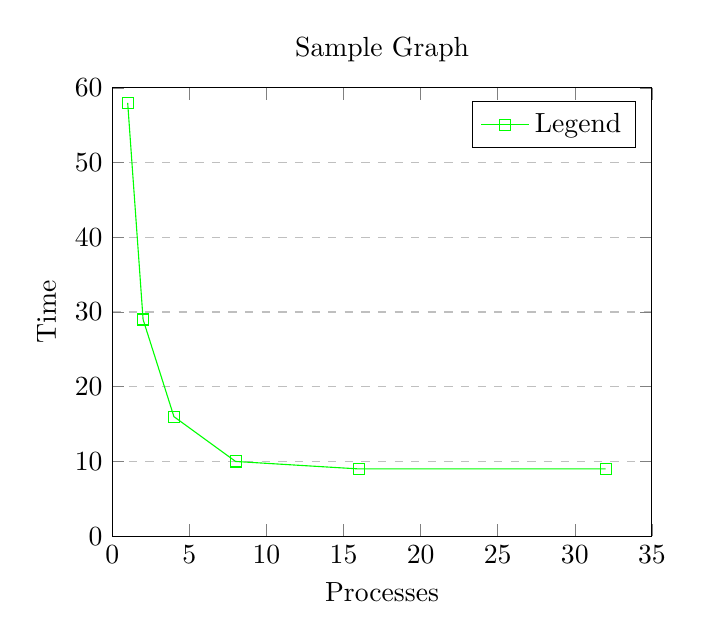
\begin{tikzpicture}
\begin{axis}[
    title={Sample Graph},
    xlabel={Processes},
    ylabel={Time},
    xmin=0, xmax=35,
    ymin=0, ymax=60,
    xtick={0,5,10,15,20,25,30,35},
    ytick={0,10,20,30,40,50,60},
    legend pos=north east,
    ymajorgrids=true,
    grid style=dashed,
]

\addplot[
    color=green,
    mark=square,
    ]
    coordinates {
    (1,58)(2,29)(4,16)(8,10)(16,9)(32,9)
    };
    \legend{Legend}
    
\end{axis}
\end{tikzpicture}


\section{Systems}
\subsection{AWS T2.Large}



%%!TEX root =  RHPC_SMPLE_UsersManual.tex

\chapter{License Information} \label{chap:LicenseInformation}
SAMPLE TRY
% CONTENTS: Harley and Lindsey will have the license information, but it may not be finalized yet.
%	\end{appendices}


\end{document}
\end

